\documentclass[tikz,border=10pt]{standalone}
\begin{document}
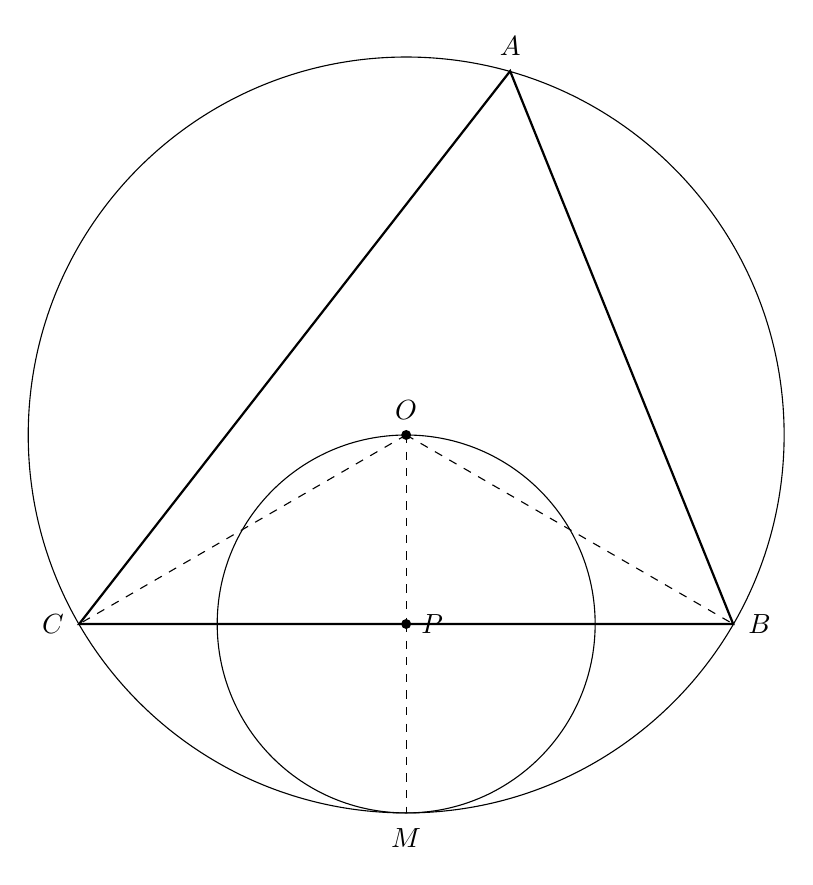
\begin{tikzpicture}[scale=1.2]
  \coordinate (O) at (0,0);
  \coordinate (M) at (0,-4);
  \coordinate (P) at (0,-2);
  \coordinate (A) at (1.1,3.85);
  \coordinate (B) at (3.46,-2);
  \coordinate (C) at (-3.46,-2);

  \draw (O) circle (4);
  \draw (P) circle (2);

  \draw[thick] (C) -- (A) -- (B) -- cycle;

  \draw[dashed] (O) -- (C);
  \draw[dashed] (O) -- (B);
  \draw[dashed] (O) -- (P);
  \draw[dashed] (P) -- (M);

  \fill (O) circle (1.5pt);
  \fill (P) circle (1.5pt);

  \node[above=2pt] at (O) {$O$};
  \node[right=2pt] at (P) {$P$};
  \node[below=2pt] at (M) {$M$};
  \node[above=2pt] at (A) {$A$};
  \node[right=2pt] at (B) {$B$};
  \node[left=2pt] at (C) {$C$};
\end{tikzpicture}
\end{document}
